% !TEX root = ./main.tex

\section{Introduction}
% \subsection{Motivation}

group theoretical methods in machine learning by Kondor \cite{kondorGroupTheoreticalMethods2008}.
diffusion kernel on graphs \cite{kondorDiffusionKernelsGraphs2002}

Many insightful and powerful models, like adiabatic quantum computation \cite{farhiQuantumComputationAdiabatic2000}, quantum random walks \cite{childsQuantumInformationProcessing2004} 
% \cite{ambainisOnedimensionalQuantumWalks2001}, 

\subsection{Preliminary and Notations}
a datum $\vbx:= (x_1,x_2,\dots,x_n) \in \realnumber^n$ is a vector where $n$ is the number of \emph{features};
dataset $\qty{\vbx^{(m)}, y}$ where the \emph{label} $y\in\qty{-1,1}$,
$\Omega$;
quantum state $\ket{z}$ with $z\in {1,2,\dots,2^n}$ where $n$ is the number of qubits,
computational basis; 
the binary representation $\ket{\vbx}=\ket{x_1,x_2,\dots,x_n},x_i\in \qty{0,1}$.
$\ket{0}^n$
% \subsubsection{Support Vector Machine (SVM)}
% \subsubsection{Kernel trick}

\subsection{SVM and Kernel trick}\label{sec:svm}
\emph{supervised learning} 
\footnote{unsupervised learning}
\subsubsection*{Support Vector Machine}
training set, test set.
training stage, classification stage.
exponentially large space;
hyperplane $(\vb{w},b)$ parametrized by a normal vector $\vb{w}\in\realnumber^n$ and a bias term $b\in\realnumber$. in the (high-dimensional) \emph{feature space}.
maximize the margin
\begin{equation}
	\arg \max_f  L(y,\tilde{y}) + \norm{}
\end{equation}
where the loss function $L$, slackness. called \emph{support vector}.
objective (cost function): \emph{empirical risk} (error rate, loss function)
\begin{equation}
	R_{emp}(\vb{\theta}) = \frac{1}{\abs{T}}
	\sum_{\vbx\in T} \probability (\tilde{y} \neq y)
\end{equation}
the dual quadratic program that (only uses access to the kernel)
we maximize 
\begin{equation}
	L_D(\alpha) = \sum_{i=1}^t \alpha_i - \frac{1}{2}\sum_{i,j=1}^t y_i y_j \alpha_i \alpha_j \kernel(\vbx_i,\vbx_j)
\end{equation}
subject to $\sum_{i=1}^t \alpha_i y_i = 0$ and $\alpha_i\ge 0$ for each $i$?.

% \begin{figure}[!ht]
% 	\centering
% 	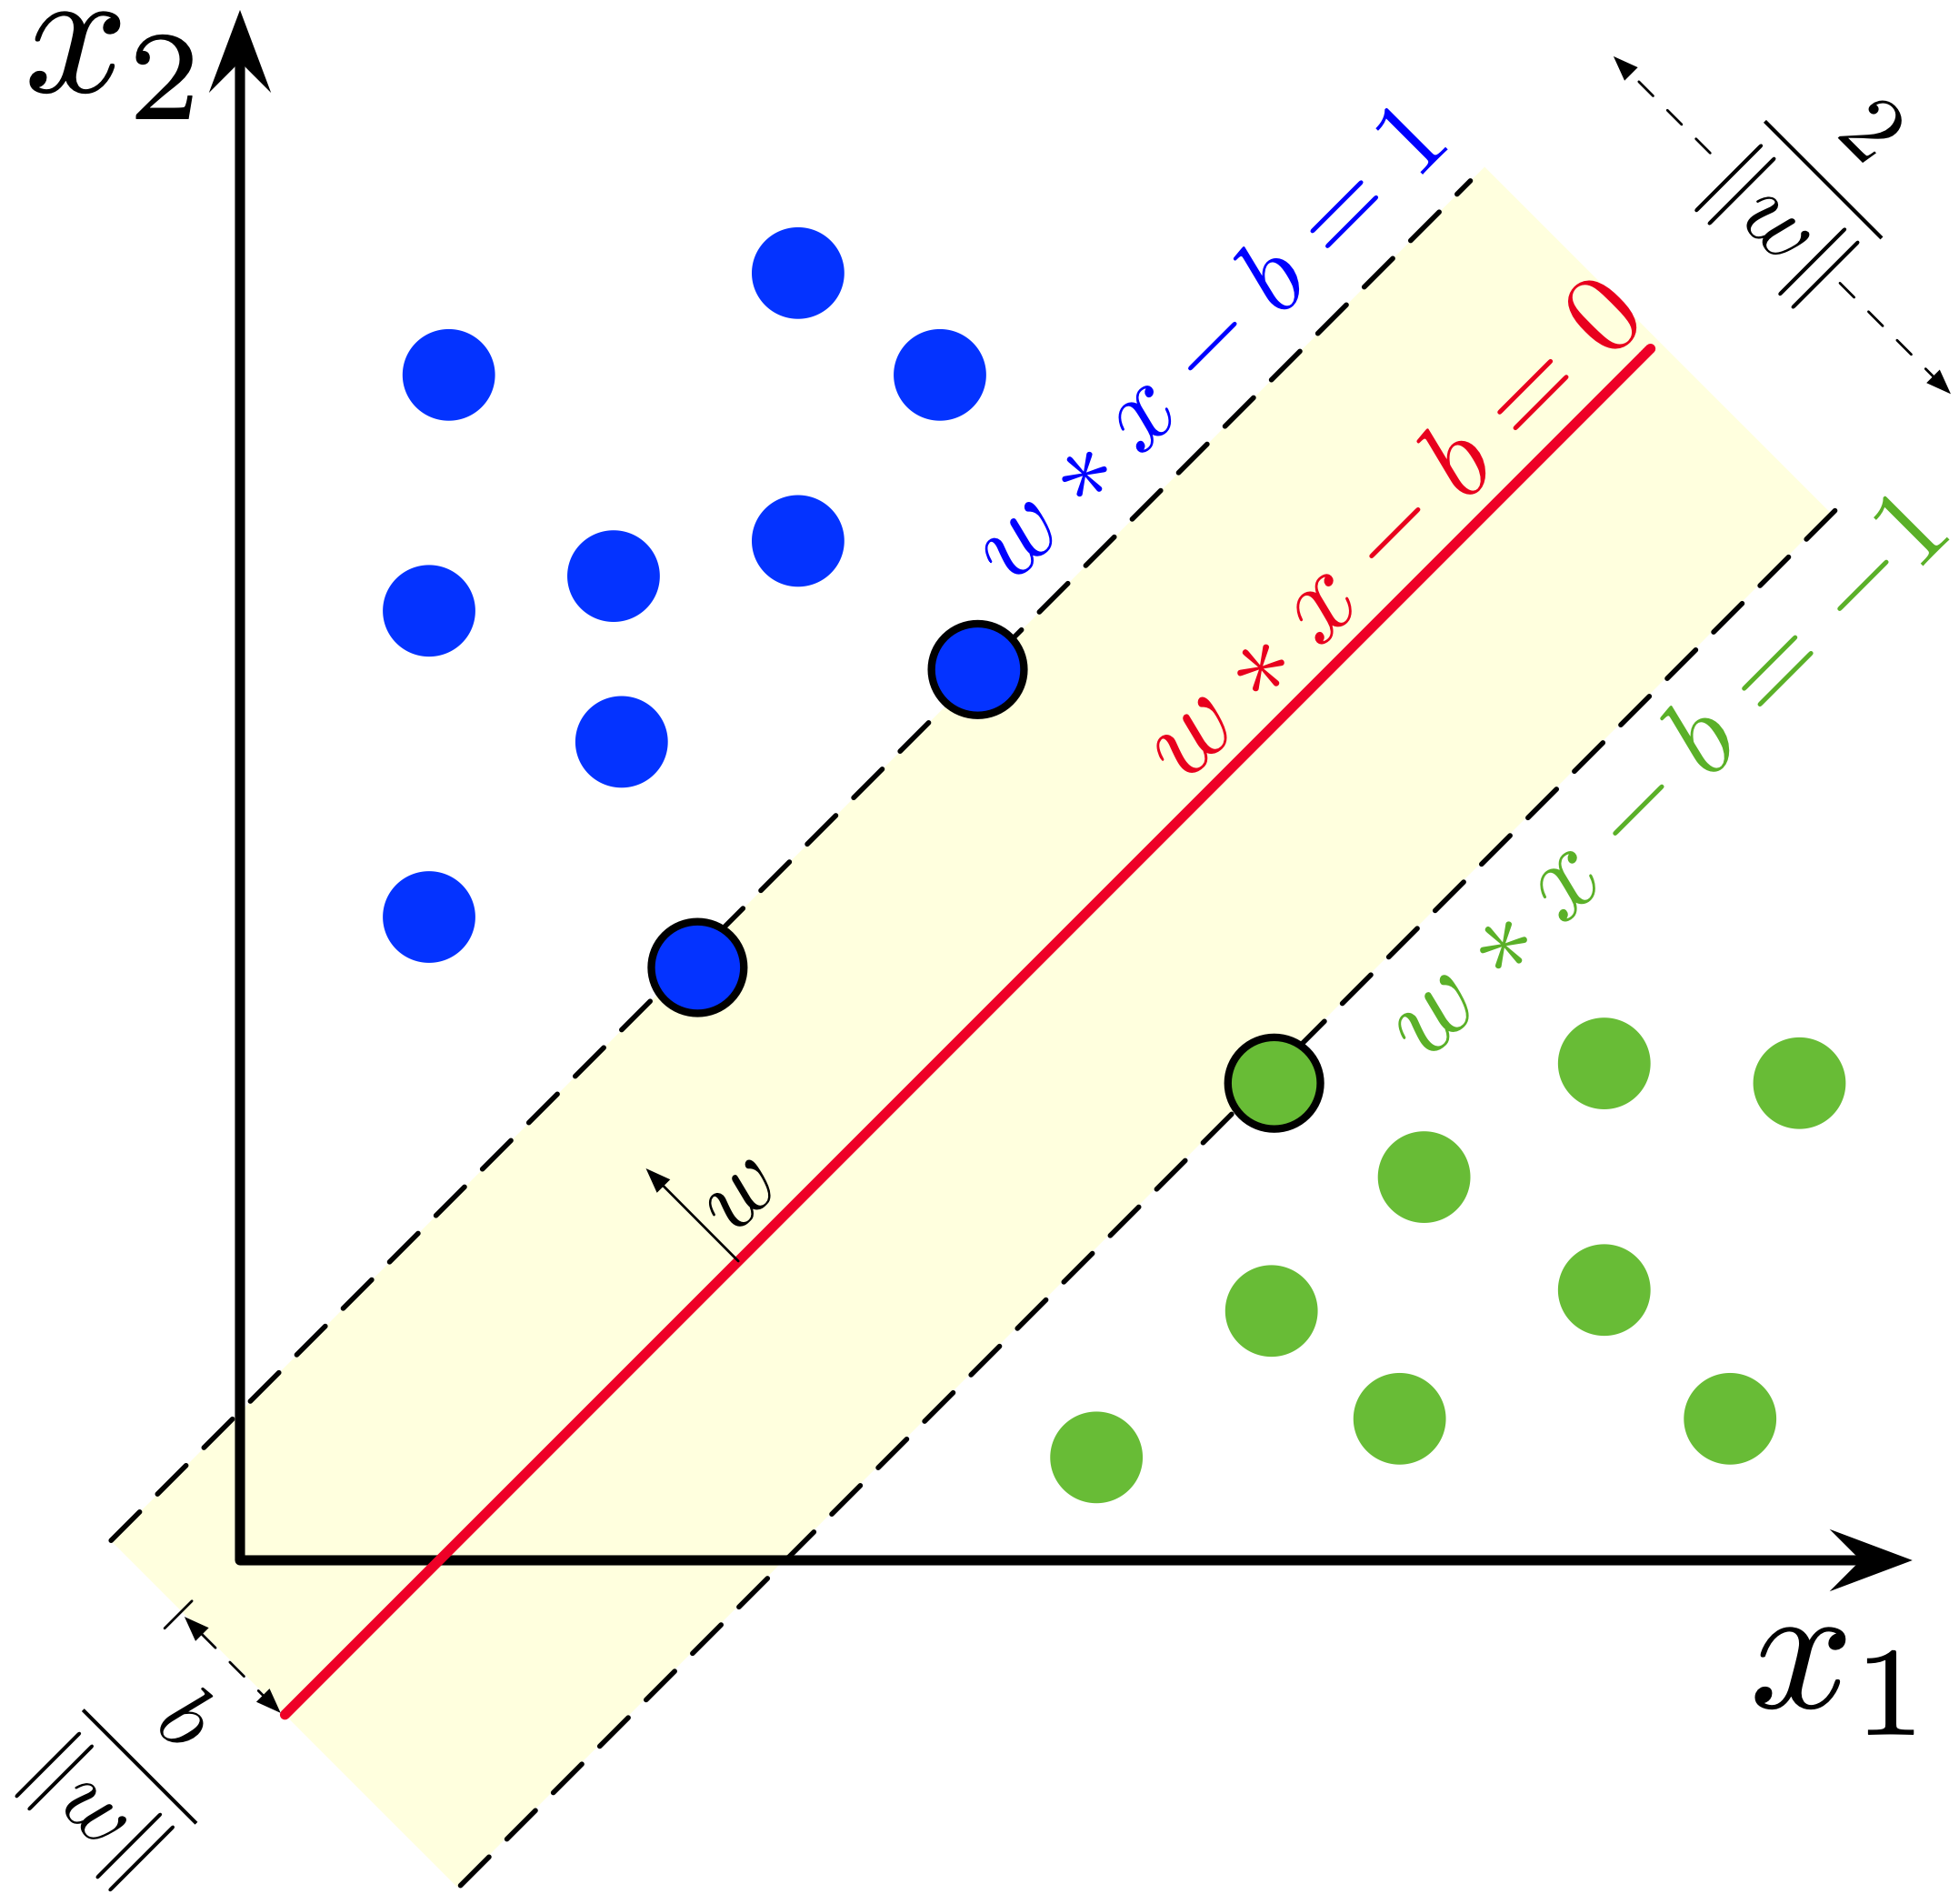
\includegraphics[width=.3\linewidth]{SVM_margin.png}
% 	\caption{}
% \end{figure}
construct the classifier
\begin{equation}
	\tilde{m}(\vb{s}) = \textup(sign) \qty(
		\sum_{i=1}^t y_i \alpha_i^* \kernel(\vbx_i,\vb{s}) + b
	)
\end{equation}

\subsubsection*{Kernel trick (method)}
\emph{kernel trick}: \emph{feature map} the input data to higher dimension such that the data are linearly separatable in this feature space.
only depend on the inner product to avoid the expensive (exponential) calculation.
a \emph{kernel function} (mapping) $\kernel: \Omega\times\Omega\mapsto\realnumber$,
a \emph{(feature) mapping} $\phi:\Omega\mapsto\hilbertspace_\kernel$
\begin{equation}
	\kernel(\vbx,\vbx') = \langle \phi(\vbx),\phi(\vbx') \rangle
\end{equation}
inner product (Dirac notation?).
\begin{definition}[Feature map]\label{def:feature_map_classical}
	\emph{feature map};
	\begin{equation}
		\Phi(\vbx) : \realnumber^n \to \hilbertspace
	\end{equation}
	from a low dimensional space non-linearly in to a high dimensional Hilbert-space $\hilbertspace$ which is commonly referred to as the \emph{feature space}.
\end{definition}
\begin{definition}[Kernel function]\label{def:kernel}
	A function $\kernel$ is a valid kernel (in machine learning) if and only if? the matrix $\kernel(x,x')$ is symmetric and positive semi-definite.
\end{definition}
\begin{figure}[!ht]
	\centering
	\begin{subfigure}{0.3\textwidth}
	\centering
		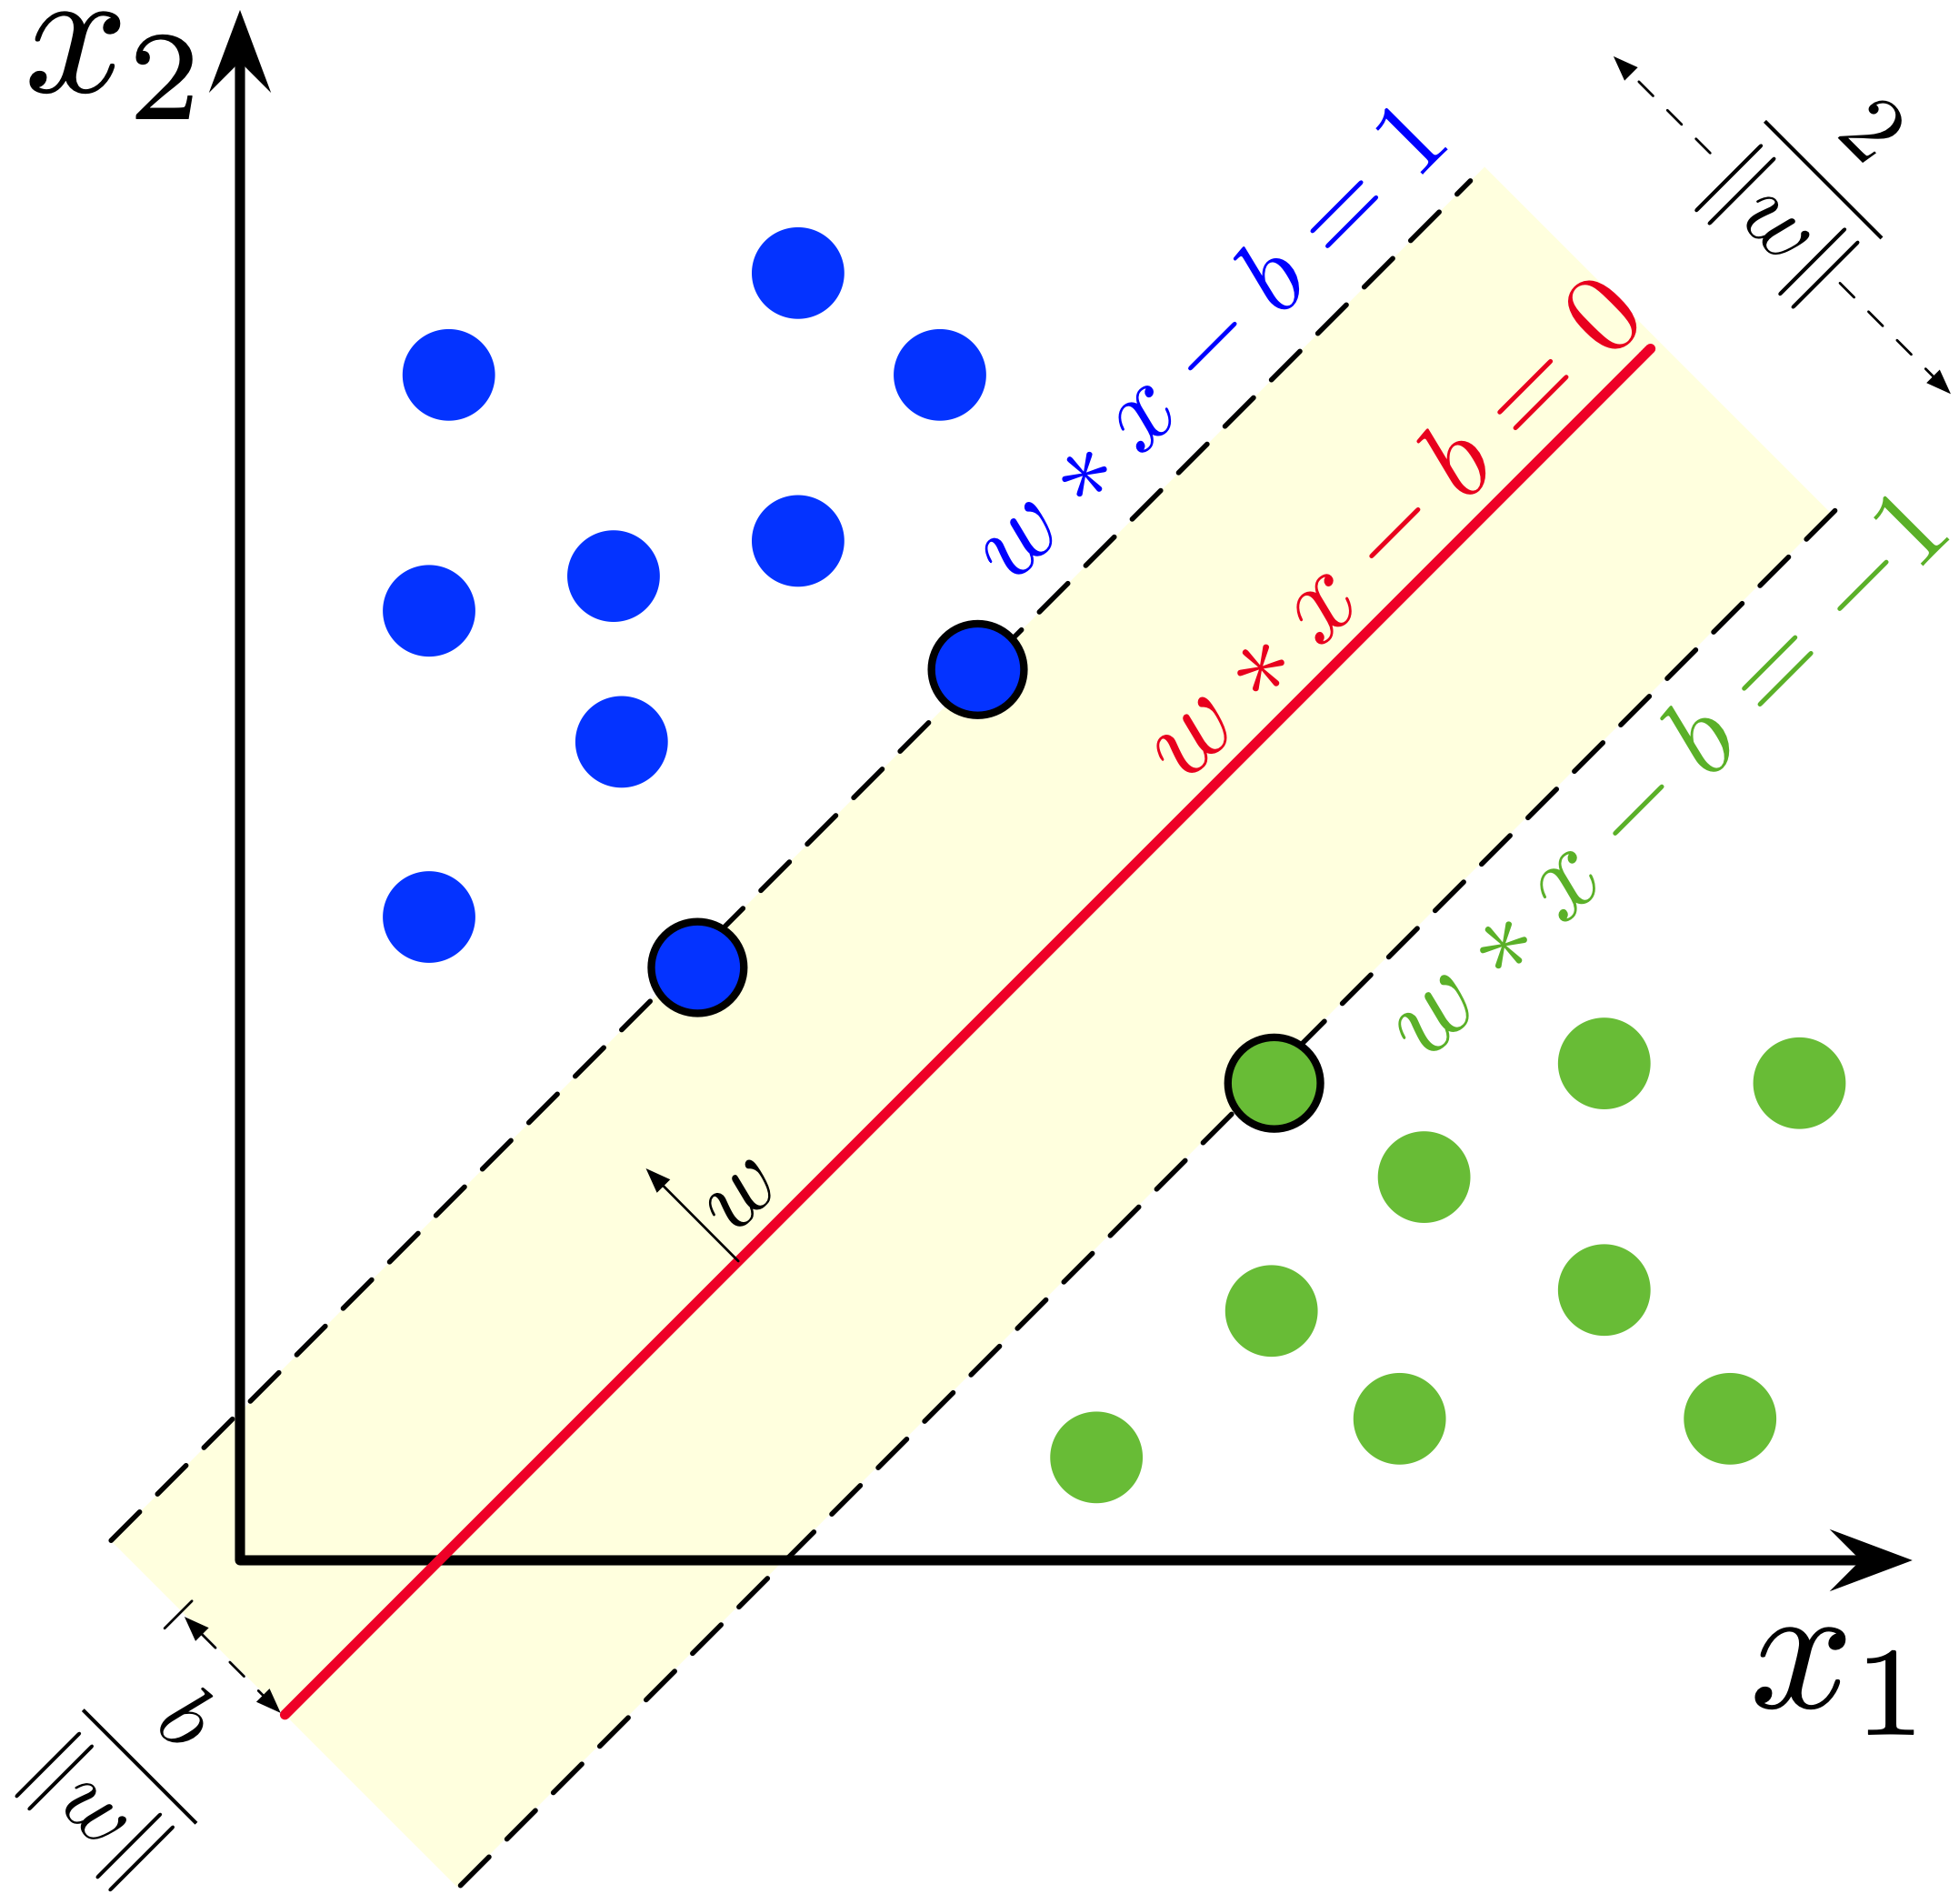
\includegraphics[width=.9\linewidth]{SVM_margin.png}
		\caption{linearly separable SVM}
	\end{subfigure}
	\begin{subfigure}{0.68\textwidth}
	\centering
		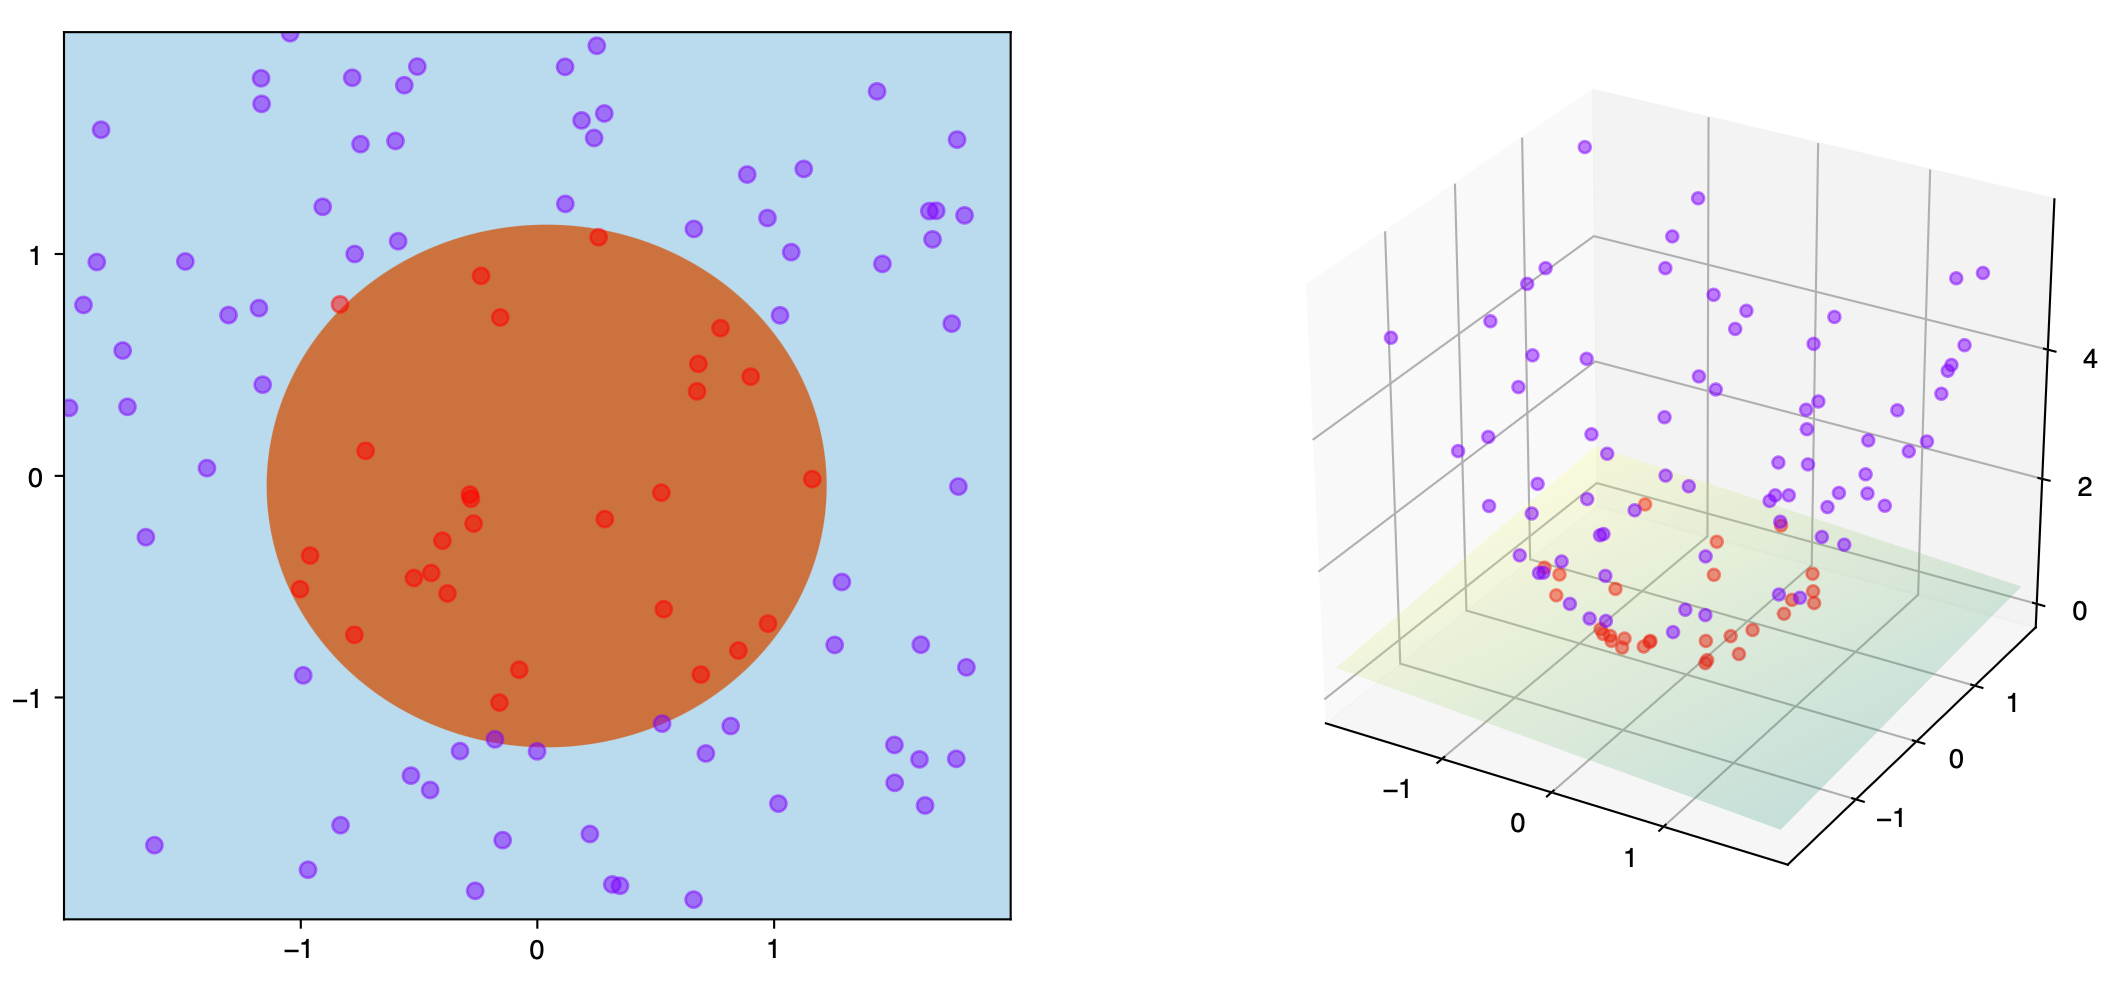
\includegraphics[width=.9\linewidth]{kernel_trick_idea.png}
		\caption{kernel trick idea: SVM with kernel given by $\phi(\vbx:=(a, b)) = (a, b, a^2 + b^2)$ and thus $\kernel(\vbx,\vb{y})=\vbx\cdot \vb{y}+\norm{x}^2 \norm{y}^2$ that only depends on inner product. The training points are mapped to a 3-dimensional space where a separating hyperplane can be easily found. (from Wikipedia: Kernel method)}	
	\end{subfigure}
\end{figure}
% \begin{figure}[!ht]
% 	\centering
% 	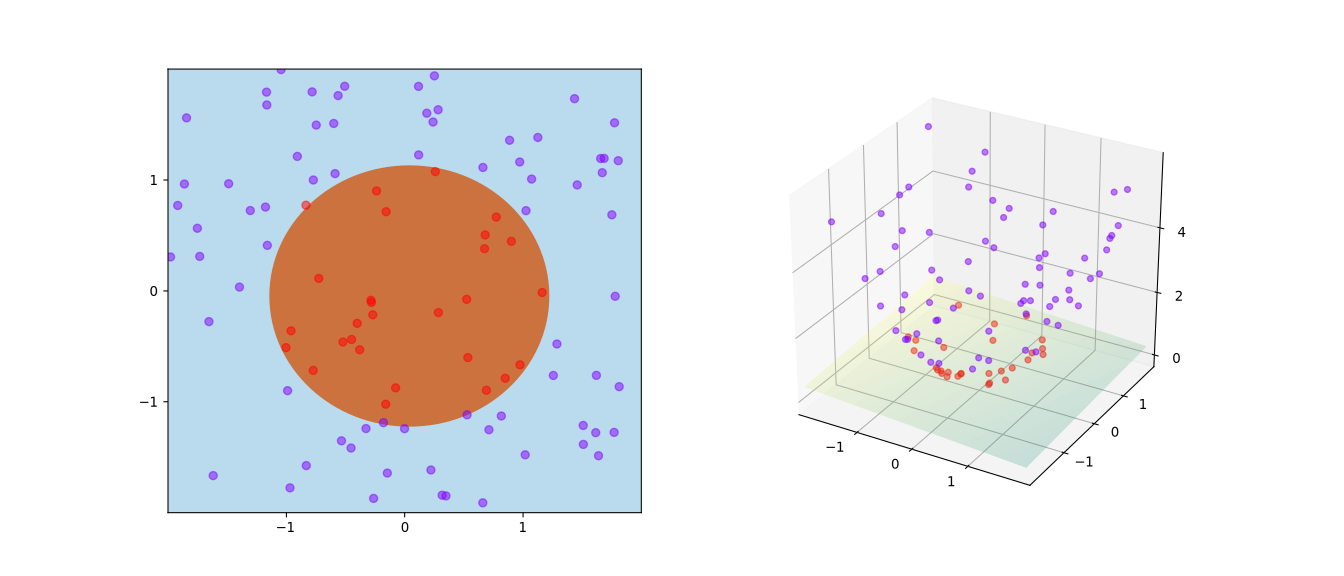
\includegraphics[width=0.8\linewidth]{Kernel_trick_idea.png}
% 	\caption{kernel trick idea: SVM with kernel given by $\phi(\vbx:=(a, b)) = (a, b, a^2 + b^2)$ and thus $\kernel(\vbx,\vb{y})=\vbx\cdot \vb{y}+\norm{x}^2 \norm{y}^2$ that only depends on inner product. The training points are mapped to a 3-dimensional space where a separating hyperplane can be easily found. (from Wikipedia: Kernel method)}
% \end{figure}
Some common kernels: 
\begin{itemize}
	\item polynomial kernel:
	\item radial:
	\item Gaussian kernel:
\end{itemize}

\begin{definition}[Reproducing Kernel Hilbert Space]
	
\end{definition}
\begin{theorem}[Representer]
	
\end{theorem}

\subsubsection*{Hilbert space}

\section{Diffusion Kernels and Continuous-Time Quantum Random Walk}

\subsection{Classical diffusion kernels on graphs}
\cite{kondorDiffusionKernelsGraphs2002}
with Euclidean space $\Omega = \realnumber^m$

\begin{definition}[Adjacency matrix]\label{def:adjacency_matrix}
	Given a (undirected, unweighted) graph $G=(V,E)$, its \emph{adjacency matrix} $\hat{A}$ is defined as
	\begin{equation}
		\hat{A}(v,v') : = 
		\begin{cases}
			1, & (v,v') \in E \\
			0, & \text{otherwise}
		\end{cases}
	\end{equation}
	where the matrix entry is 1 if the two vertices (labels of the column and the row) are connected by an edge, otherwise 0.
\end{definition}
\begin{definition}[Graph Laplacian]\label{def:graph_laplacian}
	With the adjacency matrix $\hat{A}$, the graph Laplacian is defined as
	\begin{equation}
		\llaplacian:=\hat{A}-\hat{D}	
		% \Longleftrightarrow
		% \hhat_0=\frac{\phat^2}{2m}
		% % \sim \nabla^2
		% =-\frac{\hbar^2\nabla^2}{2m}
		% % \Longleftrightarrow \dlagrangian ?
	\end{equation}
	where $\hat{D}_{vv}:=\deg(v)$ is its diagonal degree of (vertex $v$) matrix.
\end{definition}
\begin{remark}
	Graph Laplacian $\llaplacian$ is the 
	discrete version of (continuous) Laplacian operator $\laplacian$.
\end{remark}
\begin{lemma}
	exponential of i.e., $e^{\beta \hamiltonian}$ is a valid kernel
\end{lemma}

\subsubsection{Diffusion, heat equation, random walk,}
The continuous-time random walk on $G$ is defined as the \textbf{solution of the differential equation}
\begin{equation}
	\dv{t} p_j(t)
	=
	\sum_{k\in V} \llaplacian_{jk} \ p_k(t),
	\label{eq:continuous_time_random_walk}
\end{equation}
where $p_j(t)$ denotes the probability associated with vertex $j$ at time $t$
and $\llaplacian$ is \nameref{def:graph_laplacian}.

Since the columns of $L$ sum to 0
\begin{equation}
	\dv{t} \sum_{j\in V} p_j (t) = 
	\sum_{j,k\in V} \llaplacian_{jk}  p_k(t) = 0
\end{equation}
which shows that an initially normalized distribution remains normalized:
the evolution of the continuous-time random walk for any time $t$ is a \emph{stochastic process}.
\emph{random walk}, \emph{heat equation}

\subsection{Continuous-time quantum random walk}
The continuous-time quantum random walk \cite{childsExampleDifferenceQuantum2002} is the quantum analogue of classical diffusion (continuous-time random walk).
By a direct observation, \cref{eq:continuous_time_random_walk} is very similar to the time-dependent (evolution) schrodinger equation governed by a Hamiltonian operator $\hamiltonian$
\begin{equation}
	i\hbar \dv{t} | \psi \rangle = \hhat | \psi \rangle
\end{equation}
except that the factor of $i\hbar$.
\begin{definition}[Quantum propagator, kernel, transition]
	
\end{definition}

\subsection{Relation and examples}
\subsubsection{Ring (closed line)}
classical kernel 
\begin{equation}
	\kernel()
\end{equation}
\begin{figure}[!ht]
	\centering
	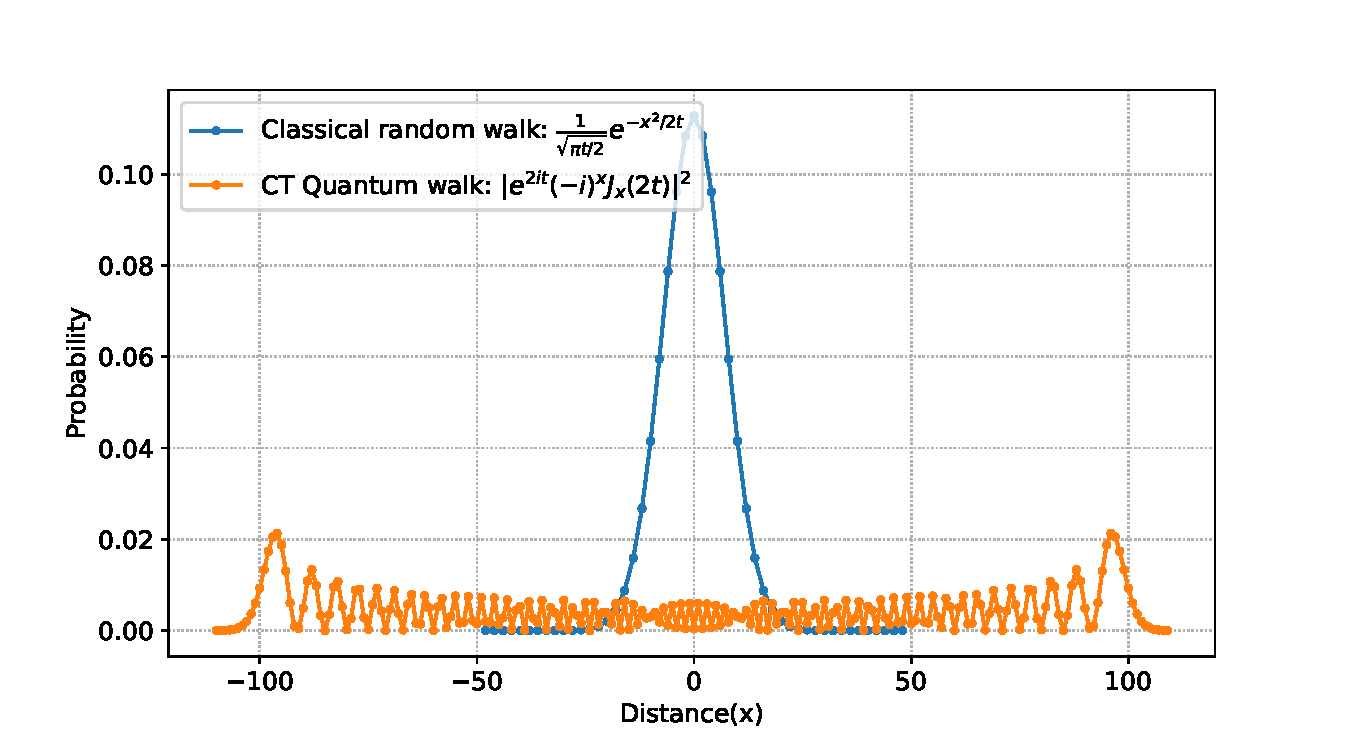
\includegraphics[width=.8\linewidth]{walk_1d.pdf}
	\caption{}
\end{figure}
quantum propagation (kernel)
\begin{align}
	\mel{z_F}{e^{-\ii t\hhat_0 }}{z_I}
	&=\sum_{p=1}^{N} 
	e^{-\ii t 2\cos(\frac{2\pi}{N}p) +\ii \frac{2\pi}{N} p(z_I-z_F)} 
	\\
	&
	% \approx \frac{1}{2\pi} \int_{\pi}^{\pi} e^{\ii p d -2\ii t cos(p)} \dd{p} 
	\approx e^{2\ii t} (-\ii)^{d} J_{d} (2t)
	\label{eq:ctqrw_kernel}
\end{align}
\begin{remark}
    The random walk on this graph starting from the origin (in either continuous or discrete time)
    typically moves a distance proportional to $\sqrt{t}$ in time $t$.
	In contrast, the quantum random walk evolves as a wave packet with speed 2.
\end{remark}

\subsubsection{Tree}
\subsubsection{Hyercube}
\subsubsection{Cayley graphs}
\begin{definition}[Cayley graph]\label{def:cayley_graph}
	Cayley graph is a graph that encodes the abstract structure of a group. 
\end{definition}

\section{Quantum Speedups via QKE}\label{sec:speedup}
A quantum version of this approach has already been proposed in \cite{rebentrostQuantumSupportVector2014},
where an exponential improvement can be achieved if data is provided in a coherent superposition. 
\begin{remark}
	However, when data is provided in the conventional way, i.e. from a classical computer, then the methods of [15] cannot be applied.
\end{remark}
input model, quantum RAM;
quantum-inspired \cite{tangQuantuminspiredClassicalAlgorithm2019}

% \subsection{Quantum Machine Learning: SVM and QKE}
\subsection{Previous works: Quantum Kernel Estimation}\label{sec:qke}
\emph{quantum kernel estimation}
\cite{schuldQuantumMachineLearning2019}
\cite{havlicekSupervisedLearningQuantum2019}
the quantum state space (Hilbert space) as the feature space to still obtain a quantum advantage
mapping the input data non-linearly to a quantum state 
\begin{equation}
	\Phi(\vbx): \Omega \to \dyad{\Phi(\vbx)},
\end{equation}
the direct quantum analogy of classical \nameref{def:feature_map_classical}

\subsubsection{Explicit method (Quantum Variational Classification)}
variational quantum circuit: generates a separating hyperplane in the quantum feature space
\begin{enumerate}
	\item $\vbx\in\Omega$ (feature) mapped to a quantum state by applying a unitary circuit $U_{\Phi(\vbx)}$ to a reference (initial) state $\ket{0}^n$
	\item a short depth quantum circuit $W(\vb{\theta})$
	\item for binary classification, apply a binary measurement $\qty{M_y}=2^{-1}(\identity + y \vb{f})$?
	\item to obtain the empirical distribution $p_y(\vbx)$, perform repeated measurement shots.
	then assign the label according to $p_y$?
\end{enumerate}

\subsubsection{Implicit method (QKE)}
estimate the kernel function quantumly and implement a conventional SVM.
Rather than using a variational quantum circuit to generate the separating hyperplane, we use a classical SVM for classification.
\begin{enumerate}
	\item the kernel $\kernel(\vbx,\vbx')$ is estimated on a quantum computer
	\item the quantum computer is used a second time to estimate the kernel for a new datum (test) $\vb{s}\in S$ with all the support vectors.
\end{enumerate}

\textbf{The kernel entries are the fidelities between different feature vectors.}
The overlap can be estimated directly from the transition amplitude 
\begin{equation}
	\abs{\braket{\Phi(\vbx)}{\Phi(\vbx')}}^2 = 
	\abs{\matrixel{0^n}{U^\dagger_{\Phi(\vbx)} U_{\Phi(\vbx')}}{0^n}}^2
\end{equation}
measure the final state in the Z-basis R-times and record the number of $\ket{o^n}$.
The frequency of this string is the estimate of the transition probability.
The kernel entry is obtained to an additive sampling error of $\tilde{\epsilon}$ when $\bigO(\tilde{\epsilon}^{-2})$ shots are used.
\emph{quantum feature map}.
quantum propagation, kernel in the path-integral formalism.

\begin{theorem}[\cite{childsExponentialAlgorithmicSpeedup2003}]
	There exists exponential separation with respect to query complexity in the adjacency matrix model
\end{theorem}
\cite{zhengSpeedingLearningQuantum2022}

\cite{liuRigorousRobustQuantum2021}

\subsection{Provable: Symmetries, graph properties, and quantum speedups}
symmetric functions rule out exponential speedup
\cite{ben-davidSymmetriesGraphProperties2020}
\subsubsection{Permutation, symmetry, and speedup}
\begin{figure}[!ht]
	\centering
	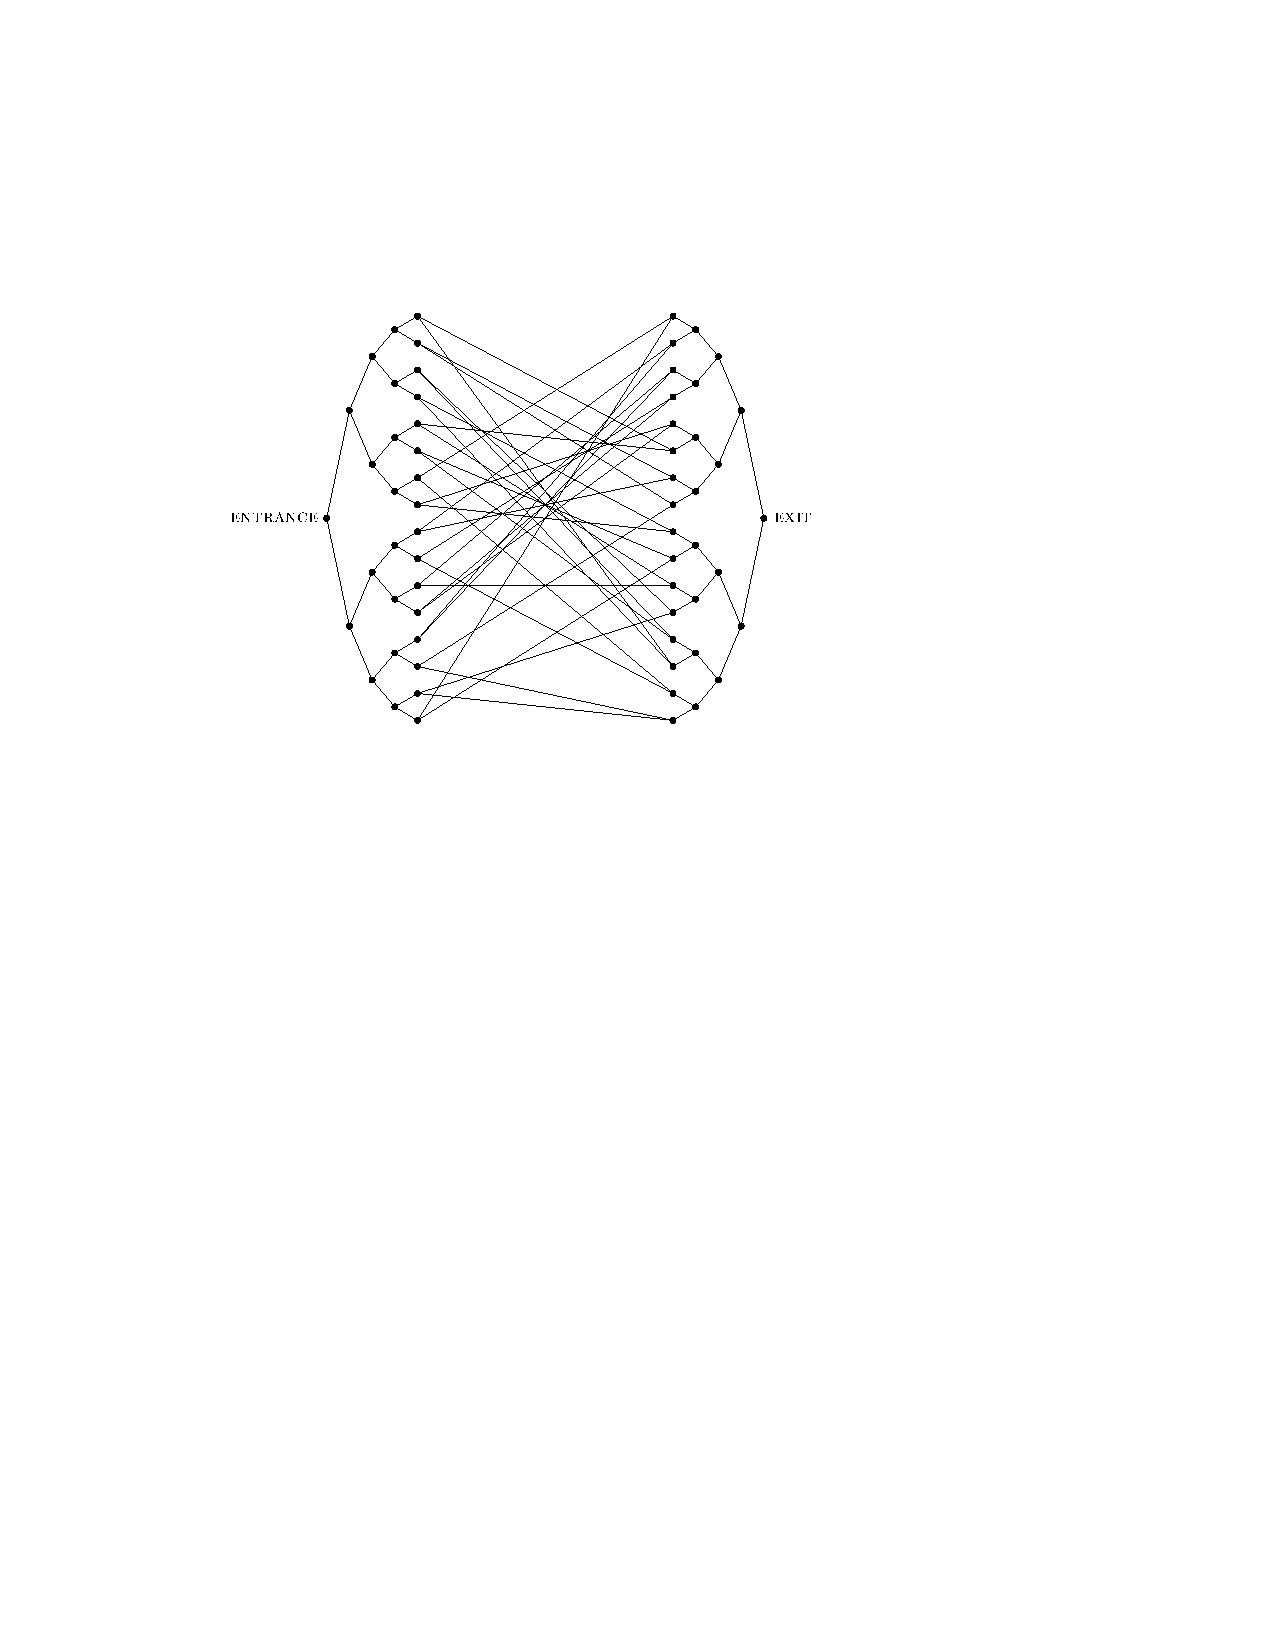
\includegraphics[width=.6\linewidth]{glued_tree.pdf}
	\caption{\cite{childsExponentialAlgorithmicSpeedup2003}}
\end{figure}

\subsection{Heuristic: Group, invariance, symmetries, physical systems}
\subsubsection{Group, symmetries in physics}
covariant 
\cite{glickCovariantQuantumKernels2021}
group theory, 
\cite{kondorGroupTheoreticalMethods2008};
symmetries in physics
\cite{bogatskiyLorentzGroupEquivariant2020};
equivariant CNN 
\cite{zhengSpeedingLearningQuantum2022}

\subsubsection{Group theory and machine learning}
\cite{kondorDiffusionKernelsGraphs2002}

\section{Experiment}\label{sec:experiments}

\subsection{Datasets and benchmark}
\subsubsection{Artificial data}
we generate artificial data that can be fully separated by our feature map.
\subsubsection{Real dataset}
JET?; quantum phase transition? order?
% benchmark

\section{Discussion and Conclusion}\label{sec:discussion}

\addcontentsline{toc}{section}{References}
\printbibliography
\appendix

\section{Machine Learning, Group Theory, and Lagrangian}
% \subsection{Kernel trick in machine learning}
% \subsubsection{SVM and Kernel}
% \subsubsection{Quantum machine learning}
\subsection{Machine learning}

\subsection{Group theory and symmetries}
\subsubsection{Representation}

\subsection{Lagrangian formalism}\label{sec:lagrangian}
\cite{xuLagrangianFormalismQuantum2021}